\documentclass{sig-alternate}
\usepackage[numbers, sort, compress]{natbib}
\usepackage{graphics}
\usepackage{graphicx}
\usepackage{epstopdf}
\usepackage{color}
\usepackage{hyperref}
\usepackage{pdfsync}
\usepackage{mdwlist}

\begin{document}
\conferenceinfo{TeraGrid '11, July 18-21, 2011, Salt Lake City, Utah, USA.} {}
\CopyrightYear{2011}
\crdata{}
%\clubpenalty=10000
%\widowpenalty = 10000


\title{Building Gateways for Life-Science Applications using the
  Dynamic Application Runtime Environment (DARE) Framework}

\numberofauthors{3}
\author{
\alignauthor Joohyun Kim\\
       \affaddr{Center for Computation and Technology}\\
       \affaddr{Louisiana State University}\\
       \affaddr{216 Johnston}\\
       \affaddr{Baton Rouge, LA} \\
       \email{jhkim@cct.lsu.edu}
\alignauthor Sharath Maddineni\\
       \affaddr{Center for Computation and Technology}\\
       \affaddr{Louisiana State University}\\
       \affaddr{216 Johnston}\\
       \affaddr{Baton Rouge, LA}
       \email{smaddineni@cct.lsu.edu}
\alignauthor Shantenu Jha\titlenote{Author for correspondence}\\
      \affaddr{Center for Computation and Technology}\\
     \affaddr{Louisiana State University}\\
      \affaddr{214 Johnston}\\
      \affaddr{Baton Rouge, LA}
     \email{sjha@cct.lsu.edu}
}

\maketitle


  % An understanding of challenges and computational requirements of
  % the life-science applications suggests that the uptake of
  % distributed heterogeneous scalable HPC resources demonstrate its
  % effectiveness as an integral component of a wide-range of
  % life-science gateways.  DARE science gateways comprise a user
  % access layer and middleware layers built upon Simple API for Grid
  % Application (SAGA) and the SAGA-based Pilot-Job (SAGA-BigJob)
  % capability.

\begin{abstract}
  This work is predicated on three important trends: (i) that the
  importance, impact and percentage of TeraGrid/XD resources assigned
  to the life sciences is increasing at a rate that is probably
  greater than other disciplines, (ii) that gateways have proven to be
  a very effective access mechanism to distributed HPC resources
  provided by the TeraGrid/XD, and in particular a very successful
  model for shared/community access models, and (iii) that in spite of
  the previous two points there are missing capabilities and
  abstractions that enable the use of the collective capacity of
  distributed cyberinfrastructure such as TeraGrid/XD, especially
  those that can be used to develop gateways in an easy, extensible
  and scalable fashion for both compute and data-intensive
  applications.  We introduce the SAGA-based, Dynamic Application
  Runtime Environment (DARE) framework from which extensible,
  versatile and effective gateways that seamlessly utilize scalable
  infrastructure can be built for a life-science applications.  We
  discuss the architecture of DARE-based gateways, and four specific
  life-science gateways -- DARE-RFOLD, DARE-DOCK, DARE-HTHP and
  DARE-NGS, that use the DARE-framework to support a wide-range of
  life-science capabilities.
\end{abstract}


% that allow a user to carry out RNA secondary structure prediction,
% virtual screening using a docking method, large-scale ensemble-based
% molecular dynamics simulations and alignment (mapping) of
% Next-Generation DNA sequencing data on a reference genome
% respectively.


%  We introduce the Distributed Adaptive Runtime Environment (DARE)
%   framework that is a SAGA-based higher-level abstraction, and
%   demonstrate its effectiveness as an integral component of a
%   wide-range of life-science gateways.  An understanding of challenges
%   and computational requirements of the life-science applications in
%   distributed heterogeneous scalable HPC resources has led to the
%   development of the DARE framework with which a lightweight,
%   extensible, versatile gateway that seamlessly utilizes scalable
%   infrastructure can be built for a life-science application
%   effectively.  DARE science gateways comprise a user access layer and
%   middleware layers built upon Simple API for Grid Application (SAGA)
%   and the SAGA-based Pilot-Job (SAGA-BigJob) capability.  This work is
%   predicated on three important trends: (i) that the importance,
%   impact and percentage of TeraGrid/XD resources assigned to the life
%   sciences is increasing at a rate that is probably greater than other
%   disciplines, (ii) that gateways have proven to be a very effective
%   access mechanism to distributed HPC resources provided by the TG/XD,
%   and in particular a very successful model for shared/community
%   access models, and (iii) that there are missing capabilities and
%   abstractions to enable the use of the collective capacity of
%   distributed cyberinfrastructure such as TG/XD, especially those that
%   can be used to develop gateways in an easy, extensible and scalable
%   fashion for both compute-intensive and data-intensive applications.
%   We present the framework and four specific life-science gateways --
%   DARE-RFOLD, DARE-DOCK, DARE-HTHP and DARE-NGS, that allow a user to
%   carry out RNA secondary structure prediction, virtual screening
%   using a docking method, large-scale ensemble-based molecular
%   dynamics simulations and alignment (mapping) of Next-Generation DNA
%   sequencing data on a reference genome respectively.

\newif\ifdraft
%\drafttrue                                                                                        \
\ifdraft
% \newcommand{\reviewer}[1]{ {\textcolor{blue}    { ***Reviewer:     #1 }}}
 \newcommand{\jkimnote}[1]{{\textcolor{green}   { ***Joohyun:   #1 }}}
 \newcommand{\jhanote}[1]{  {\textcolor{red}     { ***SJ: #1 }}}
  \newcommand{\smnote}[1]{  {\textcolor{red}     { ***Sharath: #1 }}}
 \newcommand{\todo}[1]{  {\textcolor{red}     { ***TODO: #1 }}}
 \newcommand{\fix}[1]{  {\textcolor{red}     { ***FIX: #1 }}}
 \newcommand{\reviewer}[1]{}
\else
 \newcommand{\reviewer}[1]{}
 \newcommand{\jkimnote}[1]{}
 \newcommand{\smnote}[1]{}
 \newcommand{\jhanote}[1]{}
 \newcommand{\todo}[1]{  {\textcolor{red}     { ***TODO: #1 }}}
 \newcommand{\fix}[1]{}                                                                              
 \fi



\category{D.1.3}{Software}{Concurrent Programming}{ Distributed programming/parallel programming} 
\category{J.3}{Computer Applications}{Bioinformatics}

  % We use DARE as the underlying component for four different
  % Gateways that use both TG/XD resources as well as LONI
  % The middleware, in particular, owing to the core features provided
  % by SAGA such as interoperability, distributed scale-out,
  % extensibility, adaptivity, and simplicity (IDEAS) and a pilot job
  % abstraction, SAGA-BigJob,; facilitates a gateway developer to
  % implement a various execution patterns as well as distributed data
  % management.  By employing the DARE framework as well as the
  % SAGA/SAGA-BigJob, science gateways is able to provide a target
  % scientific application whose capacity is immediately enhanced with
  % distributed scalable HPC resources such as Teragrid and other
  % emerging computing environments such as clouds, consequently
  % advancing scientific computing, for example, by providing suitable
  % solutions for challenges in data-intensive scalable computing.

% A category with the (minimum) three required fields
%\category{H.4}{Information Systems Applications}{Miscellaneous} %A  category including the fourth, optional field follows...
%\category{D.2.8}{Software Engineering}{Metrics}[complexity measures,performance measures]

\section*{General Terms}{Design,Measurement,Theory}

 \keywords{Science Gateway, Runtime Environment, Distributed Computing, Simple API for Grid
  Applications (SAGA), Pilot-Job abstraction, Data-intensive Computing}

% \keywords{ACM proceedings, \LaTeX, text
%   tagging} % NOT required for Proceedings
% \keywords{RNA conformation energy landscape, Runtime Environment,
%   SAM-I riboswitch, S gene of Bovine Corona Viral
%   Genome} % NOT required for Proceedings

%   It is interesting to note: (i) Molecular Biosciences represented
%   25\% of TeraGrid (NU) cycles used in Q1-2011.  (ii) Based on gateway
%   usage in first quarter of 20011, 3-4 of $\approx$ 20 TeraGrid
%   gateways currently are biogical/life science, which in turn account
%   for about $\approx$ 35\% of all gateway usage. (iii) However these 4
%   gateways account for about 2-3\% of recording molecular bioscience
%   usage. Points (i) - (iii) clearly imply that although a significant
%   fraction of TeraGrid cycles are devoted to Molecular Biosciences (of
%   which Molecular Dynamics is the dominant component), very few of the
%   MD users actually use gateways to access TeraGrid resources.  Given
%   the overall success and uptake of the gateways approach, prima
%   facie, there are reasons to belive that if a scalable, effective and
%   extensible capability were provided this {\it gap} could be
%   overcome. This provides an important motivation for the DARE-based
%   Science Gateways; 



\section{INTRODUCTION}

%\subsection{TeraGrid Usage by the life-science community}

The importance of computing in the life sciences has been well
appreciated. % An interesting corollary is that the rate-of-increase of
% computing resources devoted to the life sciences is increasing, and
% arguably is increasing at a rate faster than any other discipline.
In spite of fundamental limitations on the accuracy of the data, as
seen from Figs.~\ref{tg2007} \& \ref{tg2008} and Table~\ref{tg2011},
the trends are somewhat unambiguous: the percentage of TeraGrid(TG)
resources devoted to the life sciences is already more than any
discipline and the usage seems to be increasing, whether measured by
number of cycles consumed, users or allocations~\footnote{It is
  difficult to provide such information in a consistent way as the
  total number of cycles available year-to-year varies, but also which
  discipline a proposal gets assigned to is somewhat random; thus many
  chemistry proposals, even physics proposals are likely to be
  biological in nature}.

% The single largest community is the life-sciences community --
% including MD (25\%)...  Get a break-down of the total usage of the TG
% by discipline and application type.


\begin{figure}
 \centering
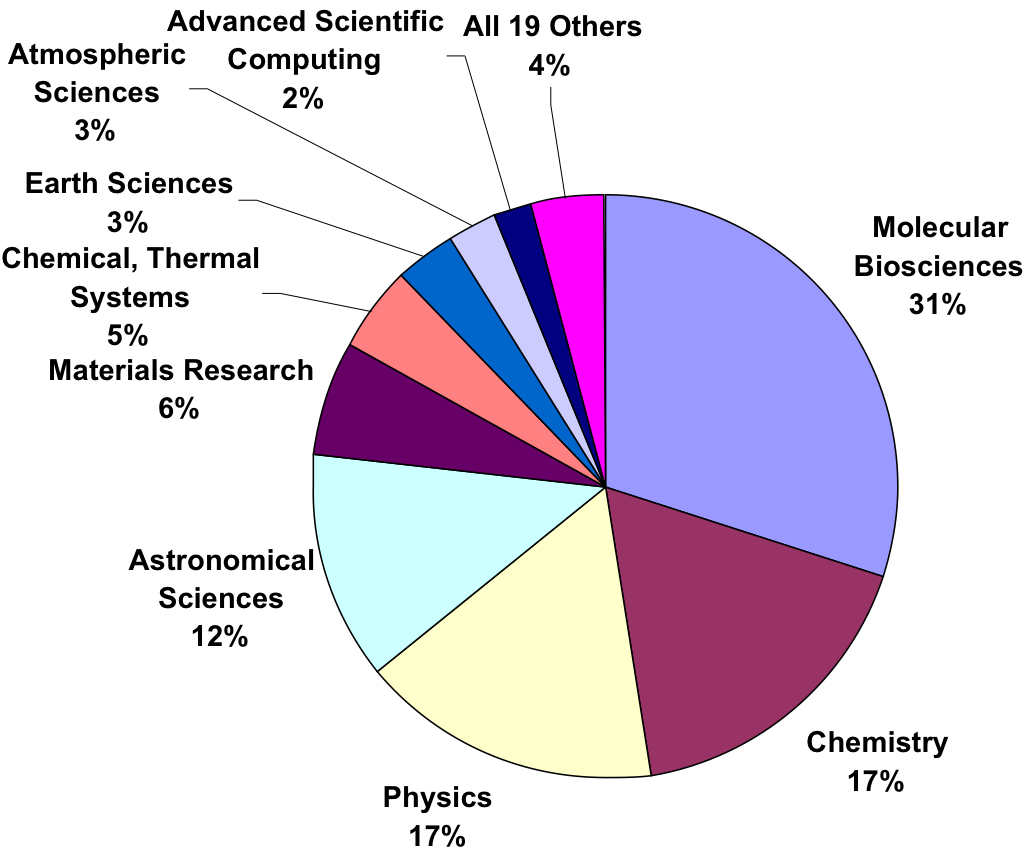
\includegraphics[scale=0.40]{figures/teragrid-discipline07}
\caption{\small 2007 Usage statistics for the TG.  (Reference
  \url{http://www.teragridforum.org/mediawiki/images/9/90/II_WorkShop_G-HPC_Nework_2009-Towns.pdf})}
  \label{tg2007}
\end{figure}


% \subsection{Large scale life-science applications on the distributed
%   HPC resources}
% Traditionally, life-science applications have been regarded as non-HPC
% applications.  Notably, only a few applications were actively pursued
% with large scale computations.  Two representative examples are
% molecular simulations and virtual docking calculations.
% Interestingly, while the former represents the case that the so-called
% scale up of bulk synchronous techniques such as MPI is used as a main
% strategy to deal with larger molecular systems, the latter represents
% the case that massive independent tasks should be carried out,
% representing two different application usage modes.


With the exception of a few applications, e.g., large-scale
simulations (mostly Molecular Dynamics(MD) ) and virtual-docking
simulations, most life-science applications have not been very
effective in utilizing HPC cyberinfrastructure.  Interestingly, MD
simulations have mostly relied on scaling-up to high core-counts,
whilst virtual docking has been dependent on high-throughput.  However
the need of large-scale distributed parallel execution for other
areas of biological/life-science applications is growing due to the
advances in experimental techniques employing high-throughput
approaches, as well as the advent of computing power and data
management capacity.  

A specific example highlighting these trends and consequent challenges
arises in the context of Next-Generation DNA Sequencing (NGS)
technologies, with unprecedented amounts of data produced through
high-throughput methods.  The volume of data arising from large genome
data sets available in public and private databases is stressing the
ability to analyze it efficiently; thus converting a data-volume
problem into a data-compute challenge, i.e., along with large data
management significant computing capacity is required to analyze the
data.

% for analyzing large volumes of data are
% effectively managed.

% required data analytics required
% along with dealing with 

Interestingly, the cyberinfrastructure considerations required to
support a broad-range of analytical approaches and at the scales
required, has received less attention than the data-management problem
and algorithmic advances.  Thus not surprisingly, traditional
production cyberinfrastructure, such as the TG, have not been used for
such data-intensive analytics and distributed applications. There are
multiple reasons, but a couple of contributing factors are: (i)
insufficient runtime environments (and abstractions) to support
concurrent computational capabilities with large-data sets to support
data-analytics (beyond visualization) in an easy, scalable and
extensible fashion, (ii) insufficient support for user-customizable
data-intensive "workflows" that effectively hide the challenges of
data-movement and efficient data-management whilst managing concurrent
distributed (computational) resources.

% Indeed, molecular simulations, virtual screening, and many other
% bioinformatics applications, particularly, regarded as the non-HPC
% applications could increase their usages dramatically by utilizing
% distributed scalable resources, which is, as presented in this work,
% addressed by a gateway development that implements a runtime
% environment for executions of target computation and distributed data
% management.

It is interesting to note~\footnote{Based upon shared
  information/private communication between SJ and Dave Hart \& Dan
  Katz}: (i) Molecular Biosciences represented 25\% of TG (NU) cycles
used in Q1-2011.  (ii) Based on gateway usage in first quarter of
20011, 3-4 of $\approx$ 20 TG gateways currently are biological/life
science, which in turn account for about $\approx$ 35\% of all gateway
usage. (iii) However these 4 gateways account for about 2-3\% of
recording molecular bioscience usage. Points (i) - (iii) clearly imply
that although a significant fraction of TG cycles are devoted to
Molecular Biosciences (of which MD is the dominant component), very
few of the MD users actually use gateways to access TG resources.
Given the overall success and uptake of the gateways approach, prima
facie, there are reasons to believe that if a scalable, effective and
extensible capability were provided this {\it gap} could be overcome.
 
\begin{figure}
 \centering
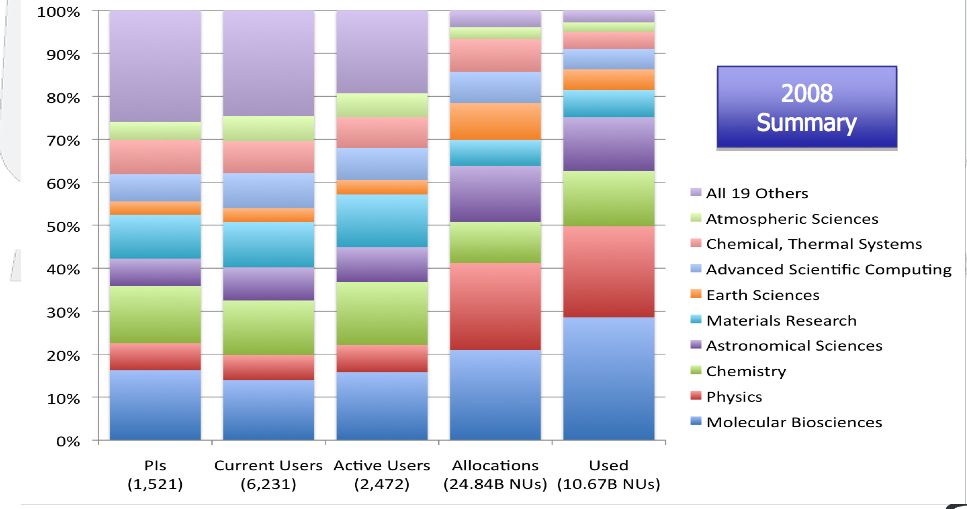
\includegraphics[scale=0.27]{figures/teragrid-discipline08}
\caption{\small 2008 Usage statistics for the TG (Reference
  \url{http://www.teragridforum.org/mediawiki/images/d/d8/DEISA-PRACE-May2009-Towns.pdf})}
  \label{tg2008}
\end{figure}

Additionally, TG Science gateways have witnessed impressive
achievements in terms of the growth of the number of supporting
researchers and computing time usages.  Those gateway developments are
often helped by suites of tools such as the Open Grid Computing
Environments\cite{ogce-2010}.  However, most gateways do not support
distributed execution, i.e., most gateways still enforce the
tight-coupling between applications and a specific resource (see
table~\ref{table:TG-sg}).  A primary reason is the additional, not
insignificant complexity to transform a target application to be able
to seamlessly utilize distributed cyberinfrastructure, and thus into a
distributed application.


% mainly due to the lack of tools for the
% coordination over multiple and distributed compute/data sites.

We observe with the advent of federated grids such as TG and its
transition to eXtreme Digital (XD) environment, such requirements
become harder to achieve as the number of connected sites and
heterogeneity will grow, as well as the computing power and the data
storage capacity of each resource reach peta or exa scales.  More
importantly, supporting a broad range of diverse execution patterns is
critical considering different application usage modes for different
life-science applications.  For example, in
Table~\ref{table:four-applications}, the usage of four life-science
applications are summarized by contrasting conventional versus
distributed modes.  Last, but not the least, it is always challenging
to respond effectively to the upcoming demands of supporting new
applications, distributed data management with new infrastructure,
implementation of novel execution patterns, which is often eased by
the development of a framework.


\begin{table}
 \small
\begin{tabular}{|c|c|c|c|c|c|} 
  \hline  Quarter & PIs & Current & Active & Allocations  & Usage\\
  & & Users  &  Users & (NUs) $\times 10^6$& (NUs) $\times 10^6$ \\ \hline
  Q3 2010 & 249 & 1,044 & 366 & 8,810   & 2,219  \\ \hline
  Q4 2010 & 254 & 1,040 & 356 & 11,720  & 2,658, \\ \hline
  Q1 2011 & 257 & 1,168 & 418 & 13,101  & 3,412\\ \hline 
\end{tabular} 
\caption{Life-Science usage of the TG over the recent
  quarters. The figures establish that both the  allocation and the
  usage of life-science applications is increasing at least in
  proportion to the increasing resource availability on the TG,
  if not faster.}
 \label{tg2011} 
\end{table}

This work is predicated on three important trends: (i) that the
importance, impact and percentage of TG/XD resources assigned to the
life sciences is increasing at a rate that is probably greater than
other disciplines, (ii) that gateways have proven to be a very
effective access mechanism to distributed HPC resources provided by
the TG/XD (and in particular a very successful model for
shared/community access models); given the landscape of the future
distributed cyberinfrastructure, we anticipate the importance of
gateways will continue to increase, and (iii) that there are missing
capabilities and abstractions to enable the use of the collective
capacity of distributed cyberinfrastructure such as TG/XD, especially
those that can be used to develop gateways in an easy, extensible and
scalable fashion for both compute-intensive and data-intensive
applications.

It is non-trivial to meet the developmental objectives for distributed
applications, viz., interoperability, distributed scale-out,
extensibility, adaptivity, simplicity -- referred to as
IDEAS\cite{ideas}.  As a modest step towards addressing point (iii),
we have shown that a flexible Pilot-Job framework can provide the
ability to run many MD simulations effectively across multiple
resources on the TG~\cite{saga-royalsoc, saga-ccgrid10}.
Specifically, we've shown how a SAGA-based implementation of the
pilot-job, supports the distributed application design objectives
categorized by the term IDEAS\cite{ideas}.

In this paper we establish how these capabilities can be generalized
and provided via gateways, to support a range of life-science
applications.  We introduce the SAGA-based DARE framework and
establish its effectiveness as an integral component for four
different life-science gateways by demonstrating that it can
effectively utilize the collective capabilities of distributed
cyberinfrastructure such as the TG/XD and LONI.

\begin{table}
 \small
\begin{tabular}{|c|c|c|c|} 
  \hline Gateway  & Type of & System  & Execution Mode 
  \\
  Name & Compu- & for a Typical & for Parallel/ \\ 
  &  tation & Task & Distributed \\
  & & & Computing \\  \hline \hline 
  
  CIPRES   & phylogeny  &  single node  & multiple  \\
   &  &   & independent   \\ 
  &  &  &  tasks \\  \hline
  GridChem   & quantum & single node or     & multiple  \\
     & chemistry, & small cluster & independent   \\
  & MD &  & task  \\ \hline
   GridAMP     & ASTEC  & legacy Domain  & pipelined \\ 
  & coupled with  &  Scientific Code   & HPC  \\
  & a parallel GE &   &  programs \\ \hline
  Nano  & portal  & large Set   & multiple \\
  Hub  & for nano- & of Tools  & independent \\
   & technology &  & tasks \\ \hline
  \hline
\end{tabular} \caption{Examples of existing TG Science Gateways. The list is not necessarily complete. More information including URLs can be found elsewhere\cite{tg-sg-list-url}.  ASTEC means Aarhus Stellar Evolution Code.}
 \label{table:TG-sg} 
\end{table}



% \subsection{Challenges in developing a gateway supporting distributed
%   applications with heterogeneous multiple HPC resources}


\section{FOUR LIFE-SCIENCE APPLICATIONS}

\begin{table}
 \small
\begin{tabular}{|c|c|c|c|} 
  \hline Science  & Supported  & Conventional   &   Distributed
  \\
  Domain & Appli- & Application & Application \\ 
  &  cation(s) & Usage Mode & Usage Mode \\  \hline \hline 
  
  Molecular   &  \texttt{NAMD} &  MPI-based  & ensemble-based   \\
  Dynamics  &  & single simulation  & multiple  \\ 
  &  & run &  simulation  \\ 
  &  &  &  runs \\ \hline
  RNA   & \texttt{SFOLD}, & short single task    & large number  \\
  Folding   & \texttt{RNAFold} & or a few serial & of tasks using   \\
  Prediction & &  tasks &distributed \\
  &  &  &   resources  \\ \hline
  NGS data     &  \texttt{BFAST} & memory-intensive  & data-intensive\\ 
  analytics  &  &  single-node   &  distributed  \\
  & & execution  & computing \\ \hline
  Virtual  & \texttt{Autodock} &  many tasks   & many tasks \\
  Screening  &  & using a cluster  & using multiple  \\
  (Docking) &  &  & resources \\ \hline
  \hline
\end{tabular} \caption{Four life-science applications of interest and their usage modes.  Four gateways were developed for these applications using the DARE framework}
 \label{table:four-applications} 
\end{table}

Here we describe the four scientific applications for which we develop
DARE-based gateways.

% briefly around the aspects primarily focused by the gateway
% development using the DARE framework

\textit{Large-scale MD simulations:} Over the past two
decades, the field of biomolecular simulation has exploded due to
increases in computational power and parallel codes, the emergence of
accurate molecular mechanical potentials or force fields and
improvements in the methods~\cite{adcock2006}. 
%\cite{amber,mackerell2008}
A continually growing body of researchers apply atomistic and
coarse-grained MD simulation methods to facilitate drug discovery,
perform advanced materials research, to design and understand
biomolecular and designed catalysts, and to provide fundamental
insight into molecular structure, dynamics and interactions.

%Particular challenges include de
%novo protein and nucleic acid folding and structure prediction;
%correctly modeling induced-fit and conformational selection as drugs
%or other molecules interact with a target macromolecule; modeling
%large ensembles of biomolecules such as proteins in a membrane
%environment, viruses, and biomolecular machines such as the ribosome;
%combined quantum and molecular mechanical treatments for modeling
%chemistry; and improving conformational sampling and estimation of
%free energies and free energy pathways. 

In response to the perceived needs and importance of molecular
simulations, numerous high performance distributed memory parallel
codes have emerged in the past two decades (e.g., NAMD, CHARMM,
AMBER, LAMMPS,GROMACS, etc.), and many now can directly include
quantum representations.  An interesting challenge in the MD community
is, along with continuing efforts that tackle more scalable molecular
systems with longer time trajectories using more powerful machines, to
develop ensemble-based simulations over multiple HPC resources.

\textit{NGS genome data analytics:} In the past several years, with
the advent NGS technologies\cite{mardis2008-tig,metzker2010}, there
has been a major paradigm shift in biological/biomedical research.
The novel capability of cost-effective resequencing, full-scale
quantitative transcriptomics, and holistic approach for cell
development and cell differentiation using protocols such as RNA-seq,
and ChIP-seq opens a completely new era for life-science
researches\cite{sorek2010}.  

In spite of such opportunities, the potential of current NGS platforms
is limited by the capacity to analyze the sequencing data generated
and the subsequent bioinformatics analysis and inference. Furthermore,
the continuing trend of reduction in sequencing costs will result in
greater volumes and a concomitant increase in the challenges of
management and analysis.  For example, current NGS platforms produce
typically billions of reads that comprise a short sequence mostly less
than 100 base pairs\cite{alex2009} and can require tens of thousands
of hours of computing time to effectively analyze.

%no sign to see the end of influx of new tools considering continuous 

There are numerous bioinformatics tools for NGS data analytics, and
thanks to continued innovation in the technologies and algorithmic
advances in such tools, there number continues to increase.  Thus a
development approach to provide these tools and capabilities is a
simple, extensibile way is important; gateways provide precisely such
a mechanism.

In the current implementation, we focus on the most important analysis
of NGS data, that is of the mapping of NGS reads on to a reference
genome.  Soon, this analysis step will be extended to support a broad
range of other analytic capabilities, such as genome variation,
genome-wide association, comparative genomics, and other applications
for investigating biological processes in a living cell.

\textit{RNA structure prediction and beyond:} Defying the old
biological dogma, positioning RNAs as a genome information
intermediate between DNAs and proteins, during the last couple of
decades, the number of scientific observations found that RNAs were
actively involved significantly in gene expression and
regulation\cite{joyce1999}. %,amaral2008}.
Now, with the well-known categories of non-coding RNAs such as miRNAs
and riboswitches, in spite of their biogenesis that does not need to
be translated into proteins, significant roles of RNAs are quite well
recognized\cite{costa2009}.
%ellington2007}. 
Importantly, RNA functions by forming required structure(s), and the
pattern of structure formation of RNAs are somewhat contrasted to
proteins that are mostly folded into highly specific 3-D
structure\cite{roth2009}. For example, riboswitches chose one of two
alternative structures, in response to metabolite binding,
consequently resulting in two different gene regulation stages, i.e.,
turning on downstream gene synthesis or turning it
off\cite{montange2008}.  Therefore, RNA structure prediction has been
the major area for RNA studies and noticeable progress was made
recently for RNA 2D structure prediction as well as 3D structure
modeling\cite{shapiro2007}.

\textit{Drug Discovery via Virtual Screening strategies:} For small
molecule drug discovery, virtual screening using a docking method has
been widely utilized and an immediate requirement for massive docking
calculations against a chemical database has been attempted by
managing such many tasks using a local cluster, HPC cluster, grids,
and clouds\cite{levesque2009,yim2010}.  The nature of required
application usage mode for virtual screening methods is a generic
example of many task computing, implying that pleasingly parallel
massive tasks carrying out a docking computation should be executed.
In spite of such well-established protocol, the challenges in drug
discovery finding putative inhibitors for target receptors are not
resolved due to intrinsic difficulties with underlying
physico-chemical models associated with the issues with scoring
function, receptor flexibility, and docking strategy itself.
Therefore, more computing power and scaled calculations by varying the
parameters for virtual screening are needed in order to understand the
accuracy of results, suggesting the need of scalable infrastructure is
highly appreciated while the application usage mode is generally
intact.

% \subsection{Computational requirements and challenges}

% A growing limitation of applications in the life sciences is that
% workflow, data management, and analysis have become rate limiting
% steps: what is missing is support for the end-to-end execution
% requirement of applications.

% In essence, the move from executing an individual task to
% \textit{large ensembles} of coupled/loosely/uncoupled tasks requires
% scientists to spend significant time on compute and data management
% problems, instead of core science.  The quantitative shift (massive
% distributed parallel compute and data resources) implies qualitative
% change in the way how life-science applications are being served for
% scientific discovery.

% We also need to move to tiered sets of computational resources.  For
% example, one can imagine running large ensembles of MD engines on
% tightly coupled parallel machines (like Ranger or Kraken) with
% real-time data streamed to separately running analysis and
% visualization resources (Lonestar, Spur), with on-the-fly monitoring
% to analyze convergence, interesting phenomena or problems.  This also
% provides the means for possible steering, for example by spawning or
% stopping separate elements of the ensemble to sample more or less in a
% particular region of interest.  In addition to real time monitoring,
% hidden correlations in the data require the saving of coarser grained
% simulation data on longer term (1-2 year) disk resources for further
% analysis and mining using less tightly coupled computational
% resources, and ultimately placing reduced and derived data sets
% seamlessly back to the campuses, archivers, and for public
% distribution.  Not only does this support the need for diverse sets of
% computational resources, large-scale storage and data transfer
% requirements for sophisticated analysis and visualization, and
% high-bandwidth networking, it also drives the need for software tools
% that facilitate the complicated workflow management, that allow
% dynamic monitoring, starting and stopping of ensemble elements without
% losing access to the global communications fabric and local
% connections, and that provide the means for facilitating data
% management and analysis.

% In essence, the move from executing an individual task to
% \textit{large ensembles} of coupled/loosely/uncoupled tasks requires
% scientists to spend significant time on compute and data management
% problems, instead of core science.  The quantitative shift (massive
% distributed parallel compute and data resources) implies qualitative
% change in the way how life-science applications are being served for
% scientific discovery.

% The quantitative shift (massive
% distributed parallel compute and data resources) implies qualitative
% change in the way how life-science applications are being served for
% scientific discovery.

\section{DYNAMIC APPLICATION RUNTIME ENVIRONMENT}

Some recurring requirements of applications in the life sciences are
the need to support the end-to-end execution requirement of
applications, i.e., integrated workflow, data management, and
analysis.  Additionally, more sophisticated execution modes are
required, e.g., move from executing an individual task to
\textit{large ensembles} of loosely-coupled or uncoupled tasks. The need
to support these requirements whilst making decisions about
scheduling, resources utilization, or workload partitioning etc, at
runtime, make these dynamic applications.

% e.g., along with the need to support runtime decisions on data
% placement, compute-workload binding etc

Currently all of the above requires scientists to spend significant
time on compute and data management problems.  To address some of
these requirements in a dynamically, and to provide the basis for
rapid development of gateways that are capable of utilizing
heterogeneous distributed computing resources in a scalable manner, we
develop the Dynamic Application Runtime Environment (DARE)
framework\cite{dareurl}.

Fig.~\ref{fig:dare-arch} represents the architecture of a gateway
based on the DARE-framework; it is comprised of the classic three
layers: (i) Access/Application Layer, (ii) Services/Middleware Layer,
and (iii) Resource, whose underlying development mechanisms are
independent and modular, but unified under the framework.

The Access/Application layer employs the open source web application
framework, pylons\cite{pylonsurl}.  The core functional layer of this
architecture -- the Services/Middleware Layer is powered by SAGA and
SAGA-based Pilot-Job capability, the
SAGA-BigJob\cite{saga-ccgrid10}. %,jha2009developing,ecmls10, ecmls11

We will show how the combination of the open-source web application
technology, the runtime environment to support the execution of
distributed applications enables the effective and quick construction
of lightweight, extensible, gateways that can utilize
distributed cyberinfrastructure. 


\subsection{SAGA and SAGA-BigJob abstraction}

We first briefly describe SAGA and SAGA-BigJob which forms a core
component of the Services/Middleware layer.
 
SAGA is an API that provides the basic functionality for developing
distributed applications, tools and frameworks\cite{saga_url}. The key
advantages of the development using SAGA include, but are not limited
to: i) to provide a general-purpose, commonly used yet standardized
functionality, while hiding complexity of heterogeneity of back-end
resources, ii) to provide building blocks for constructing
higher-level functionality and abstractions, iii) to provide the means
for developing broad range of distributed applications such as
gateways, workflows, application management systems, and runtime
environments.  Interestingly, SAGA provides a simple way to support
scripting for building distributed applications via python-binding.

SAGA-BigJob~\cite{saga-ccgrid10} was introduced as a general-purpose
pilot-job framework, with which various execution patterns and
application usage modes have been
supported~\cite{async_repex11,saga-royalsoc}.  Previously, we
demonstrated how SAGA-BigJob was able to execute scientific
applications categorized as pleasingly parallel applications and
loosely coupled applications on scalable distributed
resources\cite{jha2009developing, ecmls10, ecmls11}

Using SAGA and SAGA-based frameworks to build gateways enables the
fundamental design objectives (IDEAS) to be met efficiently and
effectively.


\subsection{Three Layers Architecture of DARE-enabled Science
  Gateways}

\begin{figure}
  \centering
  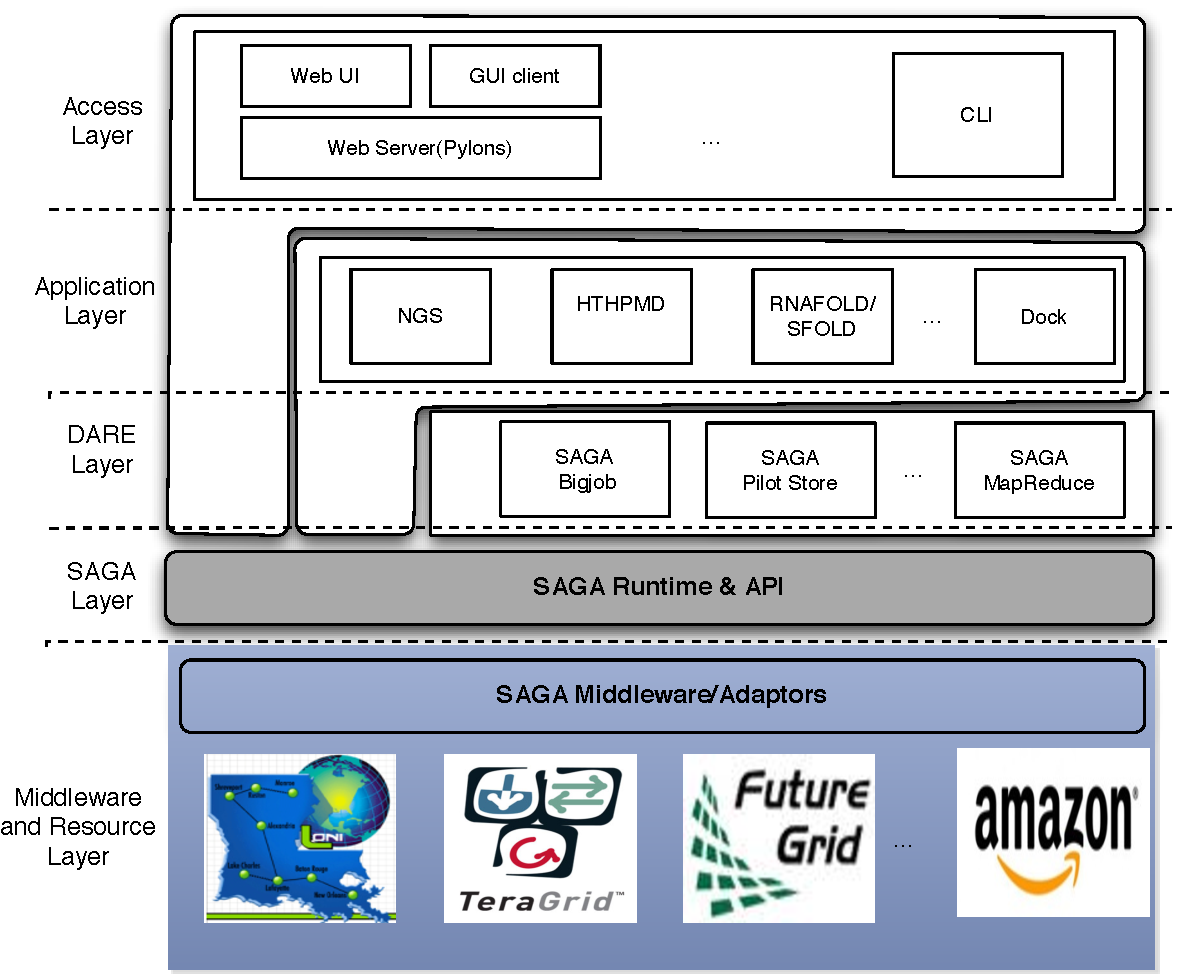
\includegraphics[scale=0.40]{figures/DAREOutline.pdf}
\caption{\small Architecture of DARE enabled science gateways }
  \label{fig:dare-arch} 
\end{figure}

\textit{Access/Application Layer:} The combination of the Access Layer
and the Application Layer is the only component a developer needs to
implement his/her own scientific logic and user interface (UI) design.
The Access Layer is composed of a web server and UI.  UI mediates the
interactions between a user and a web server, and is primarily
important for enhancing user experience.

Depending upon the type of UI, three-tier or two-tier gateways are
possible.  For example, if the web server is accessed via web pages or
a remote client, the overall architecture is regarded as a three-tier
architecture in which a user desktop, a server, and back-end resources
are independent to each other and their connection is under control by
the DARE framework.  Currently, the framework employs the use of web
UI as a primary means for a user access.  On the other hand, if
Command Line Interface (CLI) is preferred, the overall architecture
becomes two-tier, since there exist no need of a system for a remote
user.  % In the two-tier design, the server providing CLI and the back
% distributed resources are needed.

The Model-View-Controller (MVC) architecture model that underlies the
pylons web application framework\cite{pylonsurl} is very effective and advantageous in
many ways. For example, database creation, management, and transaction
are extremely simple and robust to facilitate authentication steps and
job/data creation and management by storing or retrieving related
data.  Additionally, UI creation/development and the connection
between server-side services (provided by the Services Layer) and
UI-based user interactions are also surprisingly simpler compared to
other existing approaches, requiring less programming efforts.  For
example, it is well appreciated that for a science gateway
development, the utilization of databases and server-side programming
are non-trivial tasks.

It is a developer's responsibility to find the optimal logic,
usage-mode for the target scientific application.  The Application
Layer's role is to support this responsibility, i.e., implementing the
logic and usage-mode, thus it is an important component of the
development and uptake of the gateway. As we will discuss, the
underlying Services and Middleware Layer also mitigates developmental
hassles due to reliance on SAGA/SAGA-based frameworks.

% s differ, in usage modes along with favorable execution patterns
% optimal application implemented differently with heterogeneous
% distributed resources, , which is often non-trivial if distributed
% resources and distributed data management are needed.

\textit{Services/Middleware Layer:} The challenges in building a
scalable distributed gateway is greatly mitigated by SAGA and/or
SAGA-based frameworks.  For example, by varying SAGA-BigJob
configuration, it is easy to optimize the usage of target resources
for a given computational workload and their execution
characteristics, such as pleasingly parallel, loosely-coupled, or even
multiple instances of tightly-coupled applications.  Thus once the
desired configuration have been determined, a gateway developer can
easily construct optimized runtime environment for a given target
application capable of utilizing distributed resources in a relatively
short development cycle.

% This work presents four different gateways for different life-science
% applications, once 

% One figuring out preferable application usage modes as
% well as parallelization strategies, 

% The web interface will be connected to remote job submission via a
% job scheduling and monitoring thread. This thread starts with pylons
% application and continuously communicates with local database server
% to find new jobs and it also acts as a scheduler for new jobs. Once
% this thread finds a new jobs it will start preparing the
% configuration files for that particular job from the user and
% afterwords it will start the remote job submission via application
% specific SAGA-Bigjob.
%should be carefully considered when a gateway is developed,

It is important to consider data movement requirements, since the
movement of large data sets such as input, output, temporary files is
increasingly becoming a major challenge. We have recently analyzed the
date-volumes that need to be moved around, and demonstrated some of
the challenges and solutions (for the BFAST~\cite{ecmls11} -- as a NGS
application prototype).  At the moment, GridFTP and scp are used as
the primary protocols for data
transfer. Table~\ref{table:NGS-Distributed-file} highlights the
significance of data transfer with data analytics for DARE-NGS with a
model system (human genome).

It is worth noting that with SAGA, not only can different transfer
protocols be supported, but also data-intensive programming models,
such as MapReduce and execution support for emerging infrastructure
for data-intensive computing, such as clouds can be developed and
utilized\cite{abstractions-azure,saga-ccgrid10}.  The DARE-framework
enables the simple utilization of these additional frameworks --
either as execution patterns or actual functional capabilities.

%
% All the above components are well connected but loosely coupled from
% each others as well so this provides the development of different
% kinds applications very simple and fast.

\textit{Resource Layer:} While the utilization of distributed
heterogeneous resources should be one of important motivations for a
science gateway development, most gateways currently rely on the
approaches in which multiple resource utilization is limited,
presumably, only for supporting pleasingly-parallel multiple tasks.
SAGA/SAGA-based frameworks enable distributed scale-out across
multiple production grade resources.

Various SAGA adaptors contribute to achieve interoperability for
inter-HPC-grids, HPC-cloud, and other hybrid resources.  There exist
information on how to develop a new adaptor (See SAGA web site:
\url{http://saga.cct.lsu.edu}). In addition, SAGA-BigJob adds the
capability for supporting various adaptive execution as already shown
with scientific applications such as Replica Exchange Molecular
Dynamics, hybrid CFD-MD, and NGS data
analytics\cite{saga-royalsoc,coupled,ecmls11}.

% \jkimnote{the following paragraph needs to be shorten or moved into
%   the Services Layer?}  The access layer is connected to service layer
% with the help of configuration files. The job-scheduling/monitoring
% thread which starts along with the web server is responsible for
% writing the job configuration file which changes for every single
% job. Apart from this job configuration file there are two other
% configuration files, first one has the resource list which is common
% for any application (DARE-NGS, DARE-HTHP etc. ) and the other one is
% application specific configuration on each resource containing the
% paths for executables, input, output directories. once the
% job-scheduling/monitoring thread creates the job specific
% configuration file, it invokes another thread which starts reading the
% configuration files assigned to it and acts as a manager for this
% particular job. And this thread is responsible for transferring the
% appropriate input files to different resources, submitting and running
% the required jobs requested by user and getting back the output files
% which are in turn zipped and provided to user for download via
% web. But , we have keep in mind the uploading input files and
% downloading output file via web browser has not been implemented since
% the files sizes are too big to handle via browser and we are working
% on finding ways to handle this kind of situation. SAGA plays an
% important role with this job manager thread which makes the remote job
% submission and files/folders movement across different machines very
% simple and easily usable.

 \begin{table}
\scriptsize
 \begin{tabular}{|c|c|c|c|c|c|c|} 
 \hline 
Genome & Index         & Resource    & \# of & \# of &   \# of         &	TTC  \\
  Type               & File (GB)        & &Cores &   nodes &  VMs&  (sec)\\  
  \hline
 BG &0.435& R&	64 &4&-	&1067 \\
\hline                  
BG &0.435& QB	&	64& 8&-	&719 \\
\hline
 BG &0.435&R/QB	&	32/32 &2/4& -&919 \\
\hline
 BG &0.435& FG &	64 &-&8	&712 \\
\hline
 BG &0.435 &  R/QB/ &	24/24/& 2/3 & 3 &1022\\
 & & FG& 24 &&&\\
\hline
\hline
Chr &1.9& R	&	64& 4 &-&1145 \\
\hline
Chr &1.9& QB	&	64&8&-	&924 \\
\hline
Chr &1.9& R/QB	&	32/32& 4/2&	-&1170 \\
%\hline
%HG18-Chr21 &1.9& FG	&	64	& \\
%\hline
%HG18-Chr21 &1.9& R/QB/FG	&	24(2),24(3),	& \\
%&& 	 &24(3)&\\
\hline
\hline
HG &127& R	&	256 & 16 &-	&9586\\
%\hline
%HG &127& QB	&	256 &32 &-	& \\
\hline
HG &127& R/QB	&	128/128&8/16 & -&7582 \\
\hline
\end{tabular}
\caption{
  Comparison of Time to Completion (TTC) required for the NGS data
  mapping calculations using BFAST (match step) using DARE-NGS.  
  Three genome types,
  HG18 (HG), HG18-Chr21(Chr), B. Glumae(BG) represent a human genome,
  chromosome 21 of HG18, and the genome of a microbe Burkerholderia
  Glumae.  Three compute resources are Ranger (R), QueenBee (QB), and
  FutureGrid  Eucalyptus Cloud on Sierra (FG), respectively.  The
  number of tasks for carrying out the required mapping calculation is
  30(135MB) for B. Glumae and 32(169MB)for HG18 and HG18-Chr21.
}

  \label{table:NGS-Distributed} 
\end{table}


\section{FOUR DARE-BASED GATEWAYS}
\subsection{DARE-NGS}
The DARE-NGS gateway % (\url{http://dare.cct.lsu.edu/gateways/ngs})
supports Genome-wide analysis on TG; it currently supports the mapping
process using BFAST. Mapping (alignment) is the first
step in scientific discovery utilizing NGS sequencing-based protocols
including the whole genome resequencing, RNA-seq, and ChIP-seq.  De
novo assembly without reference genome information is still in its
early stage.

It is worth mentioning that the computational complexity of the
analysis (e.g. mapping) depends, upon other things, on the size and
complexity of the reference genome and the data-size of short reads.
Given that these can vary significantly, the computational
requirements of NGS-analytics also varies (even between data-sets of
similar size).  Thus an efficient, scalable and extensible analytical
approach must be supported by any framework supporting NGS-analytics.
The current service provided by DARE-NGS focuses mainly on the mapping
step among bioinformatics tools with BFAST for single end NGS data or
BFAST+BWA for paired-end data, and eventually supports pipelines
including genome variation studies for finding SNPs and small Indels,
RNA-Seq and ChIP-Seq data analyses.

%\begin{figure}
% \centering
%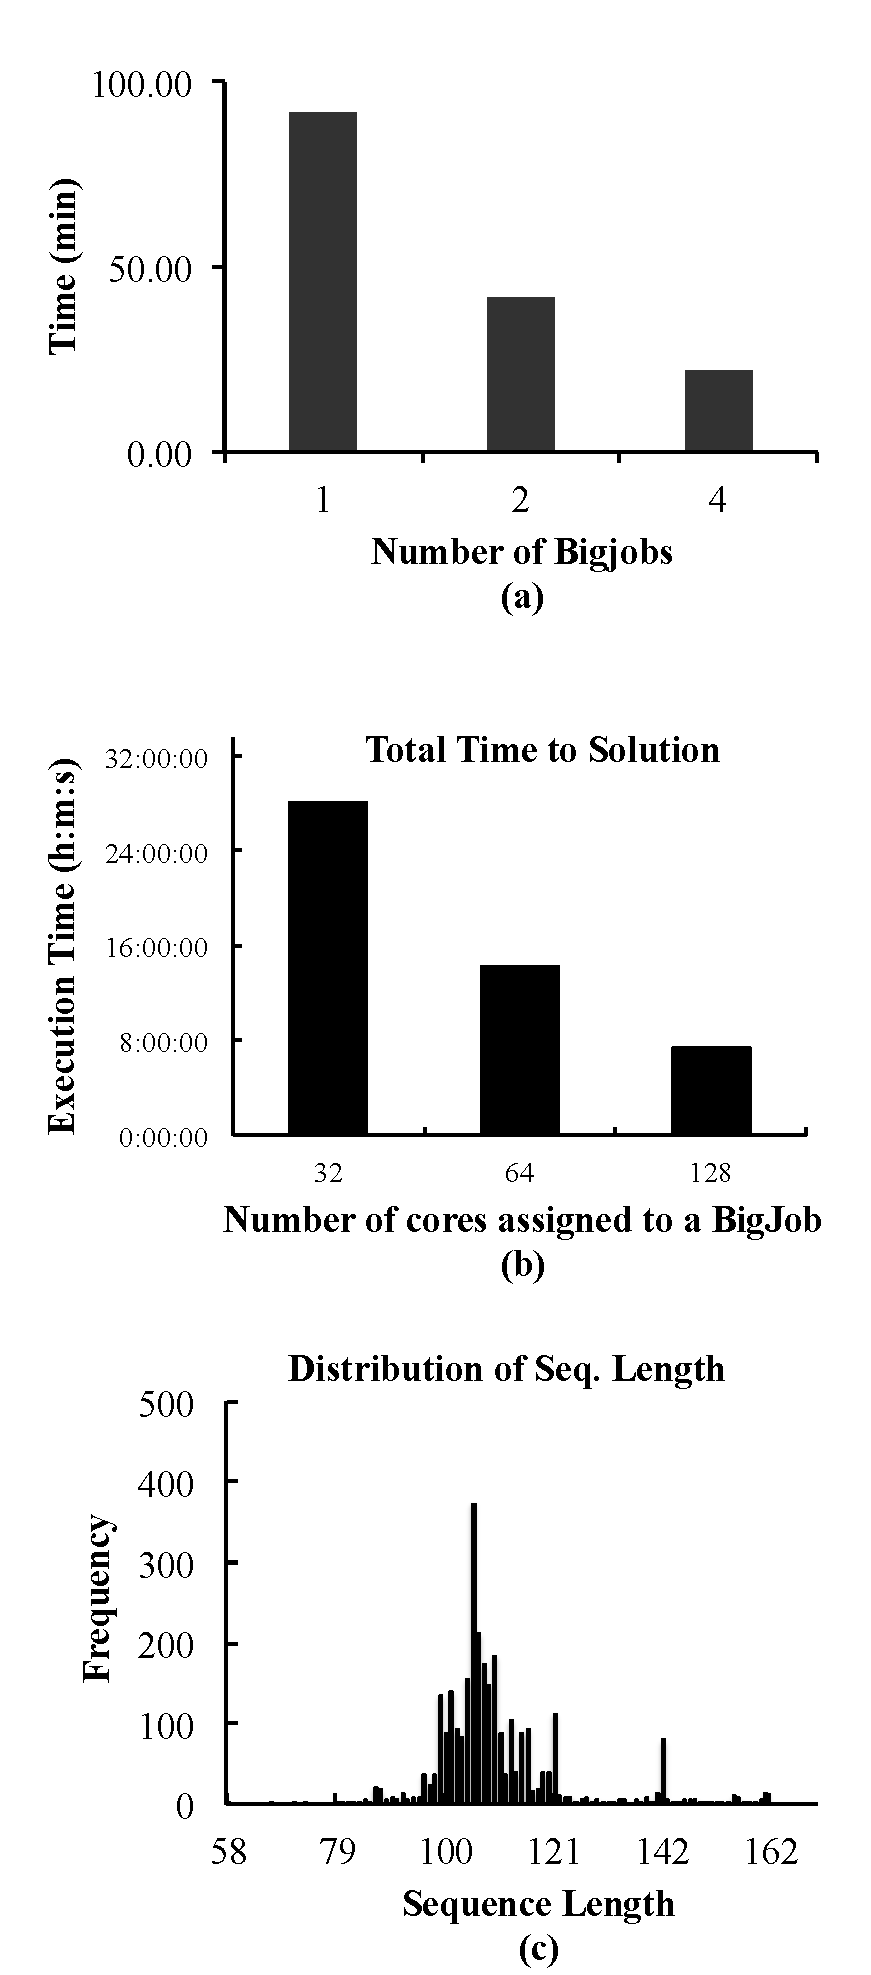
\includegraphics[scale=0.40]{figures/dare-rfold-result.pdf}
%\caption{\small Massive concurrent calculation capability is presented with the results obtained with DARE-RFOLD. The total 2910 SAM-I riboswitch sequences are injected into the DARE-RFOLD for sampling of Boltzman-weighted secondary structures.  SAGA-BigJob handles these many tasks by decoupling the resource assignment and execution of each task, collectively allowing an efficient management of many tasks. In (a) and (b), time-to-solutions with different configurations of BigJob are compared in terms of the number of BigJobs (a) and the size of a BigJob (b).  In (c), the distribution of sizes of 2910 input sequences is illustrated.  This distribution is directly associated with the distribution of time-to-solutions of all 2910 tasks. The data are taken from the recent work\cite{ccpe11}.}
%  \label{fig:dare-rfold-result} 
%\end{figure}

Recently, we reported on the exploration of NGS analytics using DARE-NGS
on HPC grids such as TG and Cloud environment of
FutureGrid\cite{ecmls11}.  Using the results obtained from such an
effort, we present the comparison of various execution scenarios with
multiple resources including a cloud system in
Table~\ref{table:NGS-Distributed}.  While this demonstrates the
capability of DARE-NGS for utilizing HPC grids and a cloud environment
together or separately, our initial results, also, indicated several
issues with an emerging distributed environment.  For example, we
observed that the large data management in FutureGrid cloud required
the Walrus data storage system but that access by multiple VM's
failed often.  

Such failures need to be managed, as human genome mapping requires
greater disk space than is often available in current (private) cloud
environments such as Futuregrid. Interestingly, we overcame some disk
space limitations, by implementing and exploiting task-level
concurrency. Nonetheless, gateway development should be flexible and
agile for future changes in resources and computing environments.

 \begin{table}
 \small
 \begin{tabular}{|c|c|c|c|c|c|c|c|c|} 
 \hline  
 	          & LW to QB (s)  & LW to Ranger(s) \\
 \hline                       
Avg. Rate && \\
MB/s & 112.04 $\pm 2$ &	    24.7 $\pm 2$  \\
 \hline                       
Index File	FTT & 1133  &	    5131.3      \\        
 \hline                       
Raw 	 Exome FTT&80.3 & 363.6\\                  
 \hline                       
Processed Short-&    & \\
Reads FTT&34&153.9  \\
 \hline                       
                    
\end{tabular}


\caption{Estimated File transfer times in seconds (FTT) with GridFTP between a local workstation (LW), QueenBee (QB), and Ranger with the case of Human Genome index files(127 GB), exome data (9 GB)and processed Short Read files (3.8 GB) . The high speed between LW (cyder located at LSU) to QB was because of the close spatial locality of the machines and LONI network which runs through LSU.   }

 \label{table:NGS-Distributed-file} 
\end{table}

For data-intensive computation such as NGS analytics, file transfer
processes are important for the total time-to-completion, and
Table~\ref{table:NGS-Distributed-file} shows such issues with the
measured transfer time obtained with DARE-NGS.  At this moment, our
gateways employ GridFTP as a default protocol on the grids such as
TG/LONI and SCP for FutureGrid Sierra Cloud.

\subsection{DARE-RFOLD}
To support nc-RNA research and broadly for the community who is
interested in the utilization of RNA structure prediction for their
research goals and education purposes, we have been developing a
gateway, DARE-RFOLD, with which a user is able to predict the Minimum
Free Energy (MFE) secondary structure or an ensemble of structure
sampled with a Boltzmann-weighted sampling scheme.

Notably, our investigation on the computational requirements of RNA
folding dynamics suggested that the support of high-throughput
computation for a large number of tasks on heterogeneous distributed
resources is beneficial for the exploration of RNA folding energy
landscape and structural characterization of SAM-I riboswitch
sequences.  As shown in recent works\cite{ecmls10,ccpe11}, the DARE
framework and its capacity for implementing a many-task-computing
support were demonstrated with the calculations of the total 2910
tasks needed for all well-known SAM-I RNA family with different
configurations for BigJob set up\cite{ecmls10}.


\subsection{DARE-DOCK}
DARE-DOCK was developed to support the basic virtual screening and for
the current implementation, the gateway supports the docking with a
popular application, Autodock\cite{autodock}.  Recently announced
Autodock-vina is used as a main tool since the application further
supports fine-grain parallelism with multi-threading multi-core
support, whose new capabilities are thus considerably suitable for a
multiple resource execution since a simple pre-processing on a target
chemical database allows to implement virtual screening on
heterogeneous distributed resources.

%\begin{figure}
% \centering
%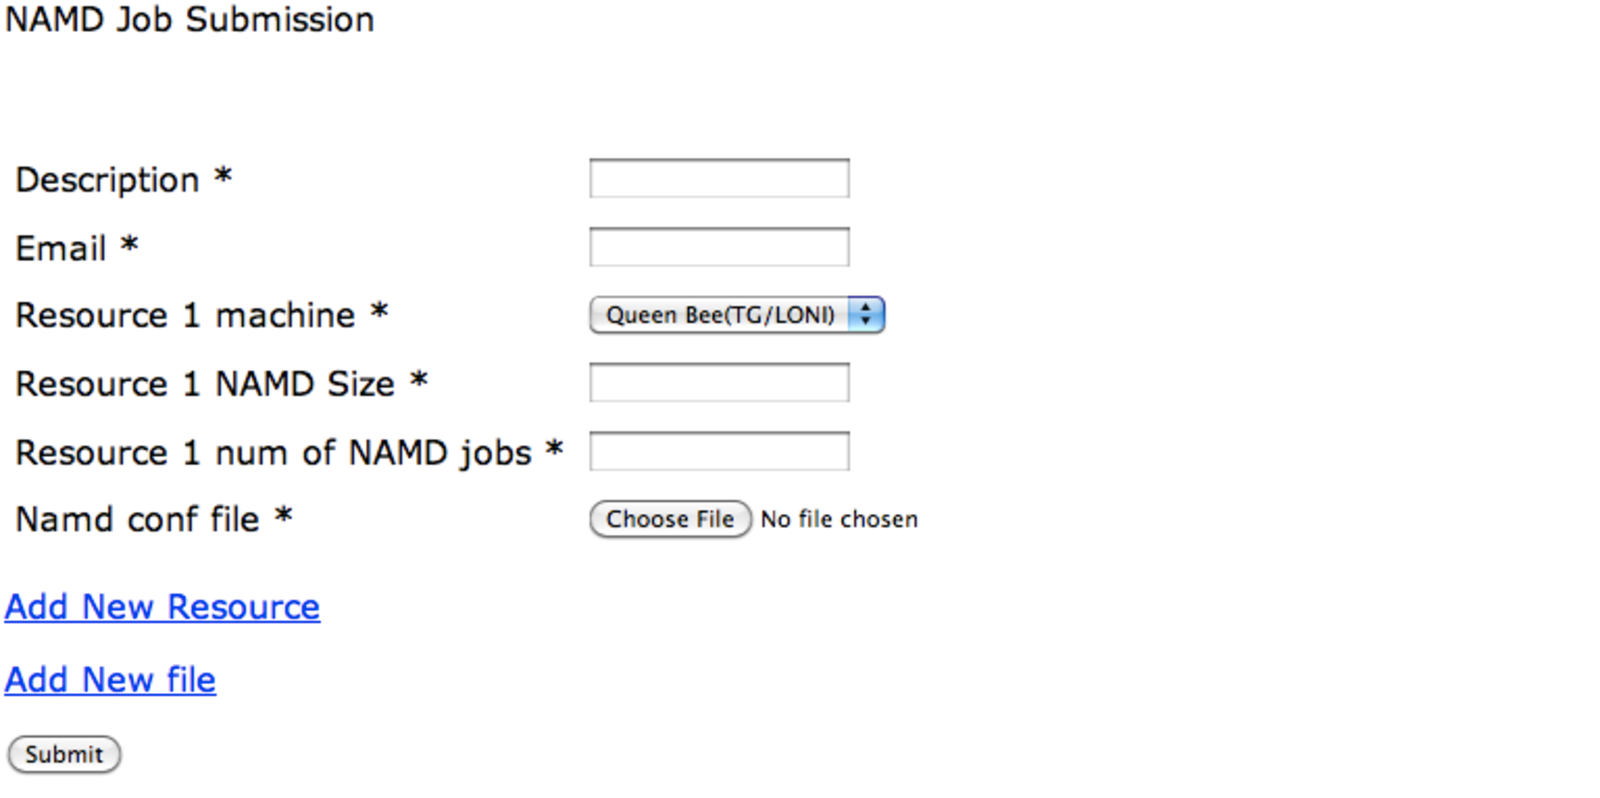
\includegraphics[scale=0.35]{figures/NAMD1.pdf}
%
%\caption{\small NAMD job submission web page form through DARE-HTHP} 
%\end{figure}

\subsection{DARE-HTHP}

An important challenge in modern biomolecular simulations, that has
received insufficient attention is not to get single long-running job
completed, but managing and executing multiple instances of the same
(or similar) physical system.  There are multiple reasons behind this
-- ranging from higher accuracy to reduced time-to-solution. For
example, multiple ensemble-member runs of the same physical system
enable better sampling In some cases, such as free-energy
calculations, multiple ensembles of the same system need to be
utilized. And even where a single long-running simulation is required,
thanks to algorithmic advances, such problems can be transformed into
the more {\it tractable} problem of solving multiple shorter run
simulations.



An ensemble simulation framework is required which has the following
characteristics: (i) Usable on a range of underlying distributed
resources and independent of resource-specific
middleware and services (i.e. scale-across), (ii) Efficiently manage
both scale-up and scale-out of ensembles -- possibly scaling up to
tens-of-thousands, if not millions of ensembles, with varying degrees
of coupling, (iii) Effective for a range of physical model sizes --
from thousands of atoms to hundreds of thousands of atoms, (iv) All of
the above without being tied to a specific underlying MD kernel, (v)
Extensible and Interoperable with emerging computational platforms
such as clouds.  Our results presented in
Table~\ref{table:HTHP-Distributed} clearly show that DARE-HTHP is able
to run such an ensemble simulations.

\jkimnote{need the attention for the following. one or two sentence
  summary would be desirable}

%When the user submits the job to run on Futuregrid cloud environment
%the input files are transferred to different VM's. The configuration
%files that are prepared in the Access/Application layer will be used
%to launch the DARE Framework which in turn starts/submits according
%to the job configuration provided by user across Grids and Clouds.

To provide the capability to run jobs in cloud using DARE, we have
prepared images which have SAGA and other required adaptors installed
along with NAMD and MPI as well.  These images are used to launch
multiple VM's and job submission similar to grid environment. Further
we are in a process of proving a capability where a user can upload
their images, and DARE will transfer them to Eucalyptus cloud on
Futuregrid and run on virtualized environment; it is also responsible
for marshaling the VM's and tasks in these environments.

 \begin{table}
\small
 \begin{tabular}{|c|c|c|c|c|c|c|} 
 \hline 
 Number           & Resource    & \# of &  \# of     &     \# of     &	TTC  \\
of tasks                &     &  Cores    &nodes&   VMs  & (sec) \\  
\hline
8& R&	64	&4 & - &141\\
\hline                  
8& QB	&	64& 8 &	-&176 \\
\hline
4/4&R/QB	&	32/32 &2/4&-&151\\
\hline
8&FG	&	64(8) & - &8&414 \\
\hline
2/3/3&R/QB/FG	&32/24/24&2/3&	3 &384\\
\hline


\end{tabular}
\caption{Time to completion (TTC) for 8 tasks of NAMD (each running on 8 cores,
  irrespective of the underlying resources), run over different resources. The three
  compute resources are Ranger (R), QueenBee (QB), 
  and  FutureGrid  Eucalyptus Cloud on Sierra(FG), respectively. The
  data shows that DARE-HTHC has been run successively on Grids and
  Clouds concurrently.}
 \label{table:HTHP-Distributed} 
\end{table}


\begin{figure}
 \centering
 \fbox{

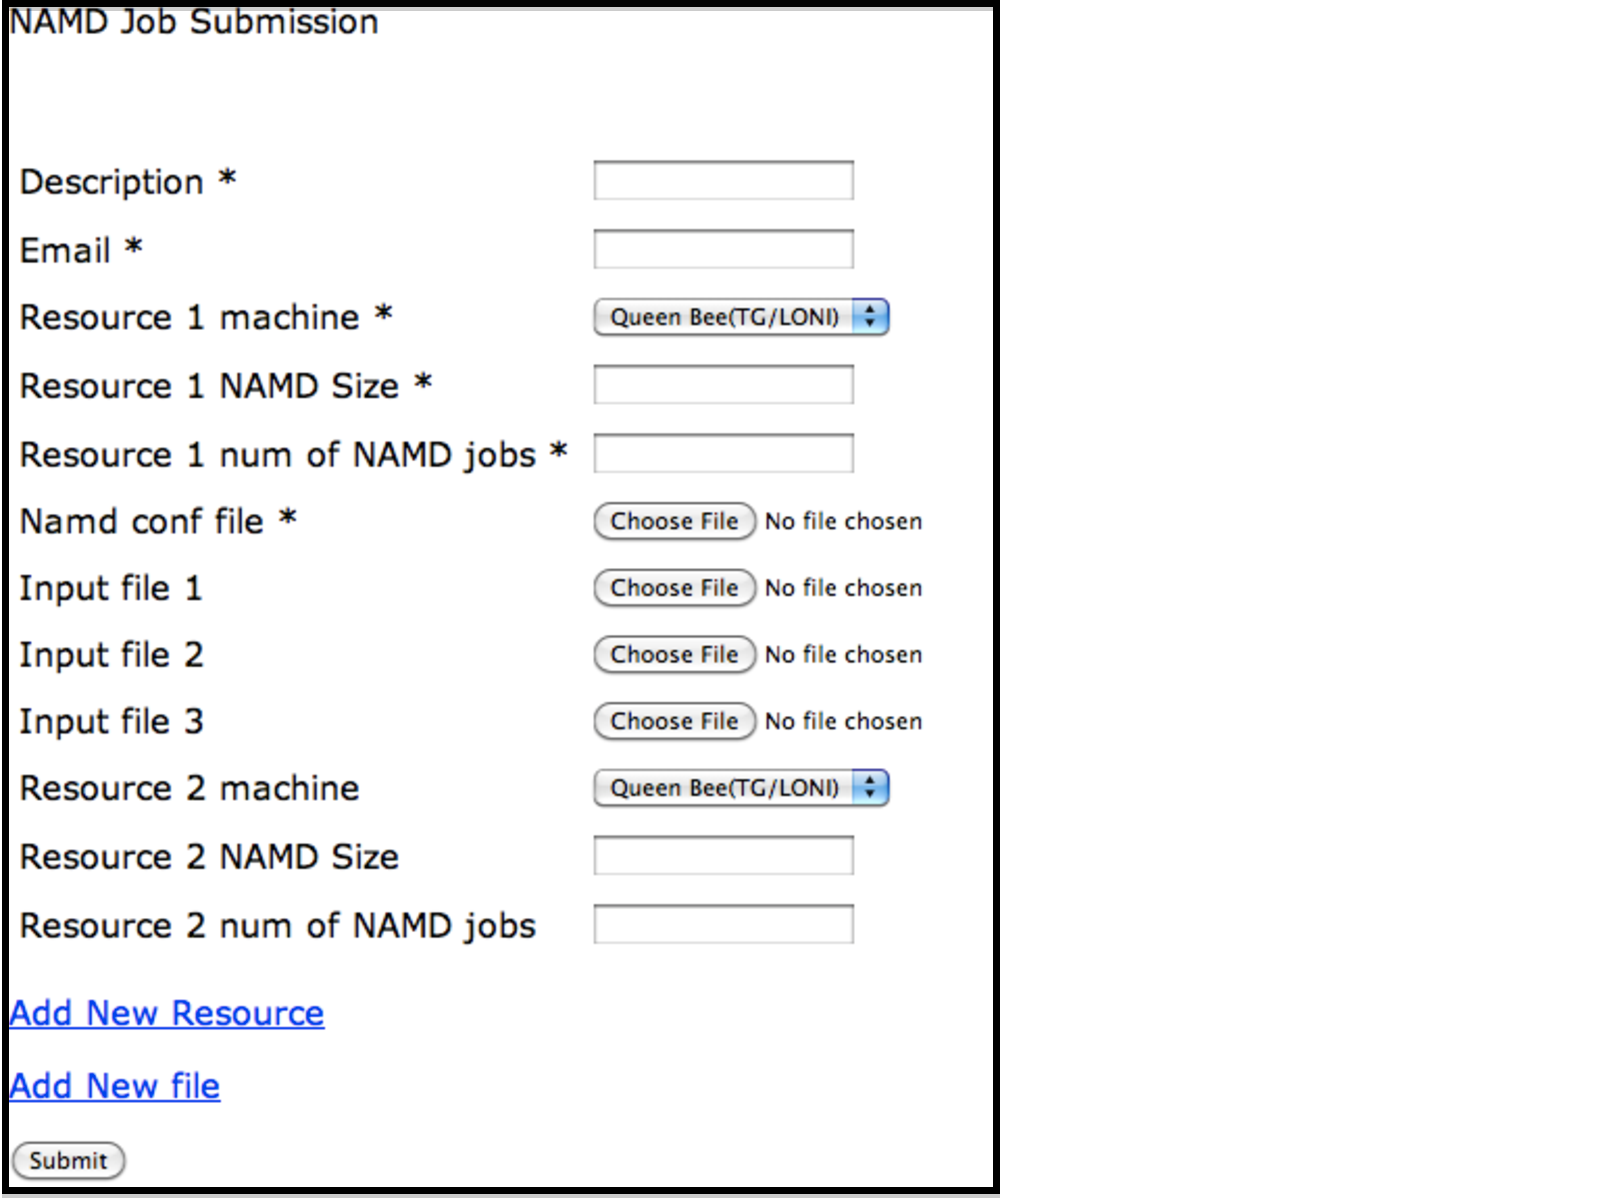
\includegraphics[scale=0.35]{figures/NAMD2.pdf}
   
  }
\caption{\small NAMD job submission web page form through
  DARE-HTHP. Here, the form indicates the usage mode with multiple
  resources.  The simple case with a single resource is default, and a
  user can expands the form by adding more resources as shown.
  DARE-HTHP can be accessed at:
  \url{http://dare.cct.lsu.edu/gateways/hthp} }
  \label{fig:NAMD2}
\end{figure}


\section{Conclusions}

All of the components in the DARE-framework are independent of each
other due to its modular structure.  The framework provides the key
functionality of job and data management over heterogeneous
distributed resources. This is provided so as to support various
execution patterns and application usage modes as well as the
full-functional access layer.  Using this template, a developer can
quickly implement his/her own scientific logic in the application
layer with python scripts.

The objective {\it Distributed scale-out} is illustrated in
Table~\ref{table:NGS-Distributed}, where two large TG systems -- QB
and Ranger, were used for the match step in BFAST pipeline.  As
demonstrated in numerous publications, having more resources and using
them collectively has multiple benefits, not least of which is the
decrease in the time-to-completion.

% It is
% noticeable that we compare different usage modes, for example, using
% one resource or two resource altogether with the same configuration
% for the computation. 

The results in Table~\ref{table:NGS-Distributed} also indicate there
are interesting aspects due to the complexity of scientific
applications.  For example, for NGS data alignment using BFAST, one
needs to determine the optimal task-level concurrency based upon how
the reference genome indexes are utilized for chunks of short read
data\cite{ecmls11}. We have also used DARE-based gateways for
efficient scale-out of multiple MD simulations in different usage
modes.

% Not only have we
% established efficient distributed scale-out for data-intensive
% applications, we have shown the effective distribution of multiple MD
% simulations-- both in loosely-coupled and uncoupled ensemble-MD
% modes.

% While SAGA via the adaptor mechanism, provides the capabilities to
% expand the infrastructure it can be utilized on, e.g., t 

Extensibility is an important objective for DARE-based gateways, and
indeed, many levels of extensibility are easily provided and utilized.
The SAGA-based approach which provide numerous adaptors to different
middleware, supports interoperability across different middleware
types; it is limited only by the availability of adaptors (SAGA has
relevant adaptors to multiple existing infrastructure including
clouds). SAGA and SAGA-BigJob, combined together,
provides great flexibility to extend scientific capability of a
gateway, e.g., support of ensemble-based simulations as a primitive
``execution unit''. With DARE-RFOLD, we provided a pipeline whereby
% for another
% capability beyond RNA secondary structure prediction.  We demonstrated
% recently that  
the output from the RNA secondary structure prediction
was utilized for Riboswitch gene annotation using structural
information. %  Furthermore, with the open source pylons framework,
% incorporation of web technologies is efficiently and easily achieved.

The design of the DARE framework supports adaptivity via the agile and
dynamic execution modes and the change of application usage modes
(e.g. concurrent multiple simulations to one large-scale simulation)
that the SAGA-based pilot-job provides.


% Note that not only varying the size of a BigJob, other possible usage
% modes supporting a case of loosely coupled applications~\cite{coupled}
% and a case of dynamically changing parallel/concurrent configurations
% in the fine-grain parallelization (for example, MPI configuration) as
% well as the coarse-grain parallelization are effectively designed.

Simplicity is provided by a well defined interface that supports
multiple {\it standards} distributed functionality, as well as
higher-level abstractions, e.g., based on the underlying SAGA-based
API, via SAGA-BigJob a general purpose Pilot-Job abstraction.

In summary, we have demonstrated how providing the right abstractions
and easy integration with other components, enables DARE-based
gateways to support the effective and easy development of science
gateway that supports distributed applications, whilst respecting the
IDEAS design-objectives.  This includes novel data-intensive
life-science applications that utilize emerging distributed
computing/data resources such as TG/XD and cloud environment
contributes.



\section{Acknowledgments}
This work is primarily supported and motivated by Grant Number
P20RR016456 from the NIH National Center For Research Resources.  We
are grateful to Andre Luckow and Ole Weidner for their work for SAGA
and SAGA-BigJob development; we also thank Ole Weidner for a
constructive criticism of this manuscript.  Computing resources used
for this work were made possible via NSF TRAC award TG-MCB090174 and
LONI resources.  This document was developed with support from the
National Science Foundation (NSF) under Grant No.  0910812 to Indiana
University for ``FutureGrid: An Experimental, High-Performance Grid
Test-bed.''. SJ would like to thank Dave Hart (SDSC) and Dan Katz
(Chicago) for helpful discussions.

%\bibliographystyle{abbrv}
\bibliographystyle{unsrt}
%\bibliography{saga,tg11}
\bibliography{tg11}
\end{document}

% As we will show in \S4, building the DARE framework on SAGA and
% SAGA-BigJob, the fundamental design objectives of IDEAS, which
% constitutes essential requirement for distributed applications, are
% achieved in a remarkably effective way.

% -- Access/Application Layer, Services/Middleware Layer, and Resource
% Layer}
